\subsection{Statistische Eigenschaften von Kontrollkarten}

\subsubsection{Interpretation von Kontrollkarten}
\begin{itemize}
	\item Zu jedem Zeitpunkt $t_i$ letzte $n_i$ der produzierten Teile entnehmen, messen, benötigte Werte berechnen und in Kontrollkarte eintragen
	\item Wenn der Prozess ausser Kontrolle ist (Punkte ausserhalb des Bereiches)
	\begin{itemize}
		\item [$\rightarrow$] Alle Teile zwischen letzter Messung und dieser Messung prüfen
		\item [$\rightarrow$] Fehler der Maschine korrigieren
		\item [$\rightarrow$] Prüfprozess beginnt wieder von vorne
	\end{itemize}
	\item Ermöglicht von Auge steigende oder fallende Tendenzen zu erkenne (indikation für systematischen Fehler)
	\item Ziel der Prozesskontrolle ist der Prozess unter statistischer Kontrolle zu halten
	\item \textbf{Western Electric Rules} zur Überwachung von Kontrollkarten, der Prozess ist ausser Kontrolle wenn:
	\begin{itemize}
		\item [1.] Ein Punkt ausserhalb von Bereich zwischen UCL und LCL liegt
		\item [2.] Zwei von drei aufeinanderfolgenden Punkten auf der gleichen Seite ausserhalb von $\frac{2}{3}$ des durch UCL und LCL festgelegten Bereich liegen ($\rightarrow$ Ausserhalb des 2-$\sigma$-Bereichs)
		\item [3.] Vier von fünf aufeinanderfolgenden Punkten auf der gleichen Seite ausserhalb von $\frac{1}{3}$ des durch UCL und LCL festgelegten Bereich liegen ($\rightarrow$ Ausserhalb des 1-$\sigma$-Bereichs)
		\item [4.] Acht aufeinanderfolgende Punkte auf der gleichen Seite der Mittellinie liegen
		\item Vorteil: Diese Regeln betrachten nicht nur einzelne Punkte sonder eine Abfolge und sucht ein Pattern
	\end{itemize}
\end{itemize}

\subsubsection{Fehler 1. und 2. Art}
\begin{itemize}
	\item \textbf{Fehler 1. Art}: richtige Nullhypothese wird abgelehnt (Detaillierte Erklärung: Skript s.29) 
	\begin{itemize}
		\item Es wird in Prozess eingegriffen obwohl dieser ungestört verläuft
		\item Wird als \textbf{blinder Alarm} bezeichnet
		\item Test der 0-Hypothese: $H_0:\mu=\mu_0$  
		\item Eine ungklücklich gewählte Stichprobe führt zum Prozesseingriff, obwohl dies nicht nötig wäre
	\end{itemize}
	\item \textbf{Fehler 2. Art}: falsche Nullyhpothese wird nicht abgelehnt
	\begin{itemize}
		\item Prozess läuft weiter, obwohl dieser derzeit gestört ist
		\item Wird als \textbf{unterlassener Alarm} bezeichnet
		\item Eine unglücklich erwischte Stichprobe führt dazu, dass Prozess weiter laufengelassen wird, obwohl dieser Fehlerhaft ist
	\end{itemize}
	\item Je kleiner $\alpha$ (Fehler 1. Art) gewählt wird, desto:
	\begin{itemize}
		\item Mehr geht die kritische Grösse $z_{1-\alpha}$ nach rechts
		\item desto kleiner wird das Risiko eine richtige Nullhypothese abzulehnen
		\item desto grösser wird $\beta$ (vom Fehler 2. Art) 
		\item desto grösser wird das Risiko für ein Fehler 2. Art
	\end{itemize}
	\item Eine Vergrösserung der Stichprobe kann obigen Problemen entgegenwirken. 
	\begin{itemize}
		\item Man spricht auch von einer Verbesserung der Trennschärfe
	\end{itemize}
	\item \textbf{Macht} Als Macht eines Tests wird die Wahrscheinlichkeit $1-\beta$ bezeichnet, mit der die Nullhypothese abgelehnt wird, wenn diese tatsächlich nicht stimmt
	\item  $\text{Macht} = P\left(\text{Entscheridung }H_0\text{nicht anzunhemen}\vert H_1 \text{sei richtig}\right)$
\end{itemize}

\subsubsection{Gütefunktion (und Eingriffsfunktion)}
\label{subsubsec:Guetefunktion}
\begin{itemize}
	\item Die Wahrscheinlichkeit die Nullhypothese $H_0$ abzulehnen, wenn $\mu_1$ vorliegt. 
	\begin{itemize}
		\item Mit anderen Worten: Den Fehler erkennen, wenn der Mittelwert $\mu_1$ abweicht vom eigentlichen Zielwert $\mu_0$
	\end{itemize}
	\item \textbf{Wahrscheinlichkeit eines unterlassenen Alarms:} $P(\delta) = 1-\tilde{g}(\delta)$
	\item Mit der normierten Variabel $\delta$ (Formel \ref{eq:delta}) messen der Abweichung vom gestörten zum ungestörten Prozess, in Einheiten von $\sigma$
	\item Gütefunktion hängt von $\mu_1$ und wird geschrieben: $g=g(\mu_1)$
	\item Wegen der Formel \ref{eq:delta} kann $g(\mu_1) = g(\delta\sigma+\mu_0) = \tilde{g}(\delta)$ festgelegt werden 
	\begin{itemize}
		\item Dabei ist $\delta$ eine Abweichung in $n\cdot\sigma$ von $\mu_0$ und $\sigma$ in der gleichen Einheit wie $\mu_0$ (z.B. \si{\milli\meter})
	\end{itemize}
	\item Die X-Achse der Gütefunktion ist in $\sigma$ und die Y-Achse ist gerade $\tilde{g}(\delta)$ 
	\item $\tilde{g}(\delta)$ wird als \textbf{Eingriffsfunktion} bezeichnet. 
	\begin{itemize}
		\item Für einen ungestörten Prozess (d.h. $\mu=\mu_0$ ) gilt $g(\mu_0) = \tilde{g}(0) = \alpha$
		\item $\alpha$ ist in Abhängigkeit vom erwarteten Signifikanzlevel (meist $\alpha = 0.0027$)
		\item Für einen gestörten Prozess sollte $g(\delta)$ möglichst gross sein
		\item Somit ist die Wahrscheinlichkeit für einen Unterlassenen Alarm ($P(\delta)=1-\tilde{g}(\delta)$) entsprechend klein
	\end{itemize}
	\item Formel \ref{eq:Phi} für die Berechnung der sich unter der Normalvertilung befindlichen Fläche
	\begin{itemize}
		\item Entspricht der Wahrscheinlichkeit ein Ergebnis in dieser Fläche zu treffen
		\item In Taschenrechner \glqq Menu $\rightarrow$ 5:Wahrscheinlichkeit $\rightarrow$ 5: Verteilungen $\rightarrow$ 2: Normal Cdf
		\item [] $\sigma$ ist dabei die Abweichung welche beim ersten $\sigma$ festzustellen ist
	\end{itemize}
	\item Operationscharakteristik: $\text{OC}(\mu_1)  = 1-g(\mu_1)$
	\begin{itemize}
		\item Stellt funktionalen Zusammenhang zwischen dem Fehler 2. Art und der Lage von $\mu_1$ her
		\item Wahrscheinlichkeit eines unterlassenen Alarmes, wenn $\mu_1$ vorliegt
	\end{itemize}
\end{itemize}
\begin{align}
	\label{eq:delta}
	\delta&=\frac{\mu_1-\mu_0}{\sigma}\qquad \Rightarrow \qquad \mu_1 = \delta\sigma+\mu_0\\
	\label{eq:Phi}
	\Phi(x,\mu,\sigma^2)&=\frac{1}{\sqrt{2\pi\sigma^2}}\int_{-\infty}^{x}e^{-\frac{\left( z-\mu\right)^2}{2\sigma^2}}\text{dz}
\end{align}

\subsubsection{Mittlere Lauflänge}
\label{subsubsec:MittlereLauflaenge}
\begin{itemize}
	\item Entgegen Kapitel \ref{subsubsec:Guetefunktion} interessieren wir uns nicht für die Wahrscheinlichkeit, dass ein Alarm bei einer einzelnen Stichprobe auftritt. Sondern wie lange es im Mittel dauert, bis wir in den Prozess eingreifen müssen. 
	\item Die Zeitspanne bis zu einem Eingriff wird \textbf{Lauflänge} resp \textbf{Run Length} genannt.
	\item Annahme Stichproben mit immer gleichem Umfang $n$ werden in regelmässige Abständen entnommen
	\begin{itemize}
		\item Wenn bei Stichprobe $i_{RL}$ erstmalig ein Eingriff nötig ist: Lauflänge ist $i_{RL}$
		\item Die Variabel $I_{RL}$ ist eine diskrete Zufallsvariabel mit der Wahrscheinlichkeit $p_k=P(I_{RL}=k)$ und $k\in\left\lbrace1,2,3,\ldots\right\rbrace$
	\end{itemize}
	\item Der Erwartungswert von $I_{RL}$ $\left( E\left(I_{RL}\right)\right)$ wird als \textbf{mittlere Lauflänge} resp. \textbf{Average Rung Lenght} bezeichnet, kurz \textbf{ARL}
	\begin{itemize}
		\item Diese beschreibt mittlere Zeitspanne bis Eingreifen in den laufenden Prozess nötig ist
		\item Hängt von Mittelwert $\mu_1$ und den Kontrollgrenzen ab
		\item Ein Prozess wäre ideal, wenn bei $\mu=\mu_0$ kein blinder Alarm auftritt (und somit kein Eingreifen nötig ist)
		\item Das Ereignis $I_{RL}=k$  tritt ein wenn der erste Eingriff bei der $k.$ Stichprobe erfolgt
		\item Mit Parameter $p$ (Formel \ref{eq:ParamP}) als Eingriffswahrscheinlichkeit (Wahrscheinlichkeit das Kontrollgrenze überschritten) haben wir:
		\begin{itemize}
			\item Wahrscheinlichkeit des Ereignises bei Stichprobe $k$ in Formel \ref{eq:geomverteilung}
			\item Der Erwartungswert der Variabel $I_{RL}$ in Formel \ref{eq:Erwartungswert}
		\end{itemize}
	\end{itemize}
	\item Für die mittlere Lauflänge folgt somit Formel \ref{eq:ARL2}. 
	\begin{itemize}
		\item Reminder: $\delta$ = Vielefaches für $\sigma$ gemäss Anforderungen an Prozess, 
		\item z.B. Wenn Irrtumswahrscheinlichkeit $\alpha = 0.0027$ ist, ist $\delta = 3$, siehe Anhang \ref{Anh:WichtigeSigma}
		\item Wenn ein ungestörter Prozess vorliegt ($\mu_1=\mu_0$, somit $\delta=0$) $\tilde{g}(0)=\alpha$
	\end{itemize}
\end{itemize}
\begin{align}
\label{eq:ARL}
\text{ARL} &= E\left(I_{RL}\right) = \sum_{k=1}^{\infty}kp_k\\
\label{eq:ParamP}
p &= p(\mu_1) = P(\mu\leq \text{LCL})+P(\text{UCL}\leq\mu) = g(\mu_1) = \tilde{g}(\delta)\\
\label{eq:geomverteilung}
p_k&= p(1-p)^{k-1}\\
\label{eq:Erwartungswert}
E(I_{RL}) &= \frac{1}{p}\\
\label{eq:ARL2}
\text{ARL}(\delta) &= \frac{1}{p(\mu)} = \frac{1}{g(\mu_1)}=\frac{1}{\tilde{g}(\delta)}
\end{align}

\subsubsection{Beispiel Guetefunktion und ARL}
\begin{figure}[!h]
	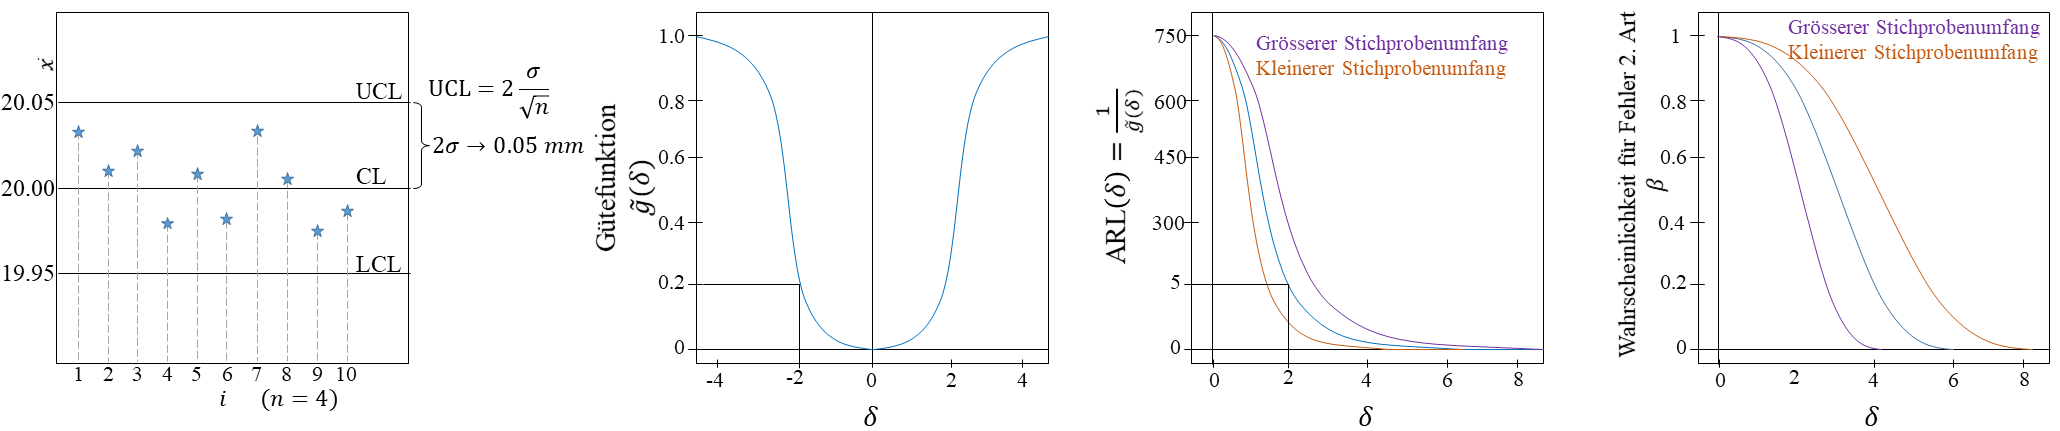
\includegraphics[width=1\linewidth]{figures/Guetefunktion3.png}
	%\caption{}
	\label{fig:guetefunktion}\\
	\begin{minipage}{1\linewidth}
		\begin{align*}
			\mu_0 &= \SI{20.000}{\milli\meter}\\
			\sigma &= \SI{0.05}{\milli\meter}\\
			n&=4\\
			\text{Irrtumswahrscheinlichkeit} &: \alpha = 0.0455\\
			\Rightarrow  & 2\sigma \text{ Aus Tabelle in Anhang \ref{Anh:WichtigeSigma}}\\
			\text{UCL/LCL}&: \mu_0\pm 0.05\\
			\sigma = 2\sigma &\rightarrow \delta=2\\ 
			\Rightarrow \tilde{g}(\delta) &= \tilde{g}(2)=0.2\\ 
			\Rightarrow \text{ARL}(2) &= 5 
		\end{align*}
	Benötigte Werte in Abh. $\delta$ aus Diagrammen lesen
	\end{minipage}
\end{figure}

\subsubsection{Prozessfähigkeit}
\begin{itemize}
	\item \textbf{Prozessbereich}: Wenn zulässiger Bereich $\left[\mu_0-3\sigma, \mu_0+3\sigma\right]$ ist, ist Prozessbereich $6\sigma$
	\begin{itemize}
		\item Achtung:Kontrollgrenzen (UCL und LCL) sind abhängig von Stichprobenumfang und nicht somit nur bei $n=1$ identisch mit Prozessbereich
	\end{itemize}
	\item \textbf{Toleranzgrenzen} USL und LSL sind bei Fertigung einzuhalten
	\item Die \textbf{Toleranzmitte} (SL) Mittelwert Zwischen oberer und unterer Toleranzgrenze
	\item Der \textbf{Prozessfähigkeitsindex} (PCR) drückt Verhältnis zwischen Breite des Toleranzbereiches und Breite des Prozessbereiches aus
	\item Unter der Annahme, dass Prozess unter Kontrolle ist ($\mu_1 = \mu_0$ und SL$=\mu_0$) gilt:
	\begin{itemize}
		\item PCR $= 1 \rightarrow$ Ausschussquote von genau $\alpha$ liegt vor
		\item PCR $< 1 \rightarrow$ Ausschussquote von mehr als $\alpha$ liegt vor. Prozessfähigkeit nicht vorhanden
		\item PCR $> 1 \rightarrow$ Ausschussquote von weniger als $\alpha$ liegt vor. Prozessfähigkeit vorhanden
	\end{itemize}
	\item Achtung: Wenn Zielwert $\mu_0$ und Prozessstreuung $\sigma$ nicht bekannt ist (der Normalfall), reagieren diese Schätzungen sehr empfindlich auf, wenn Prozess nicht unter Kontrolle ist, oder keine Normalverteilung der Messgrösse vorliegt
\end{itemize}
\begin{align}
	\text{SL} &= \frac{\text{USL}+\text{LSL}}{2}\\
	\text{PCR} &= C_p = \frac{\text{USL}-\text{LSL}}{6\sigma} \qquad \text{Achtung: 6 hängt ab von gegebner Irrtumswahrscheinlichkeit }\alpha \text{, hier }\alpha=0.0027\\
\end{align}

\newpage

